\documentclass{article}

\usepackage{graphicx}
\usepackage{systeme}
\usepackage{mathabx}
\usepackage[T1]{fontenc}



\title{Lab 9}
\author{Filip Jędrzejewski}

\begin{document}
	\maketitle
	
	\section*{Zadanie 1}
	
	\subsection*{Opis problemu}

	Celem zadania było przedstawienie każdego z poniższych równań różniczkowych zwyczajnych jako równoważny układ równań pierwszego rzędu.

	\subsection*{Równanie Van der Pol’a}

	\begin{equation}
		y'' = y' (1-y^2)-y
	\end{equation}

	Zapiszmy:

	\begin{equation}
		y_1 = y
	\end{equation}

	\begin{equation}
		y_2 = y'
	\end{equation}
	
	Zatem:

	\begin{equation}
		\left\{\begin{array}{rcl}
			y_1'&=&y_2\\
			y_2'&=&y_2(1-y_1^2)-y_1\\
			\end{array} \right.
	\end{equation}


	\subsection*{Równanie Blasiusa}

	\begin{equation}
		y''' = -yy''
	\end{equation}

	Zapiszmy:

	\begin{equation}
		y_1 = y
	\end{equation}

	\begin{equation}
		y_2 = y'
	\end{equation}

	\begin{equation}
		y_3 = y''
	\end{equation}


	\newpage

	Zatem:

	\begin{equation}
		\left\{\begin{array}{rcl}
			y_1'&=&y_2\\
			y_2'&=&y_3\\
			y_3'&=&-y_1y_3
			\end{array} \right.
	\end{equation}


	\subsection*{Prawo powszechnego ciążenia dla problemu dwóch ciał o dużej różnicy mas}

	\begin{equation}
		\left\{\begin{array}{rcl}
			y_1''&=&-GM \frac{y_1}{(y_1^2+y_2^2)^{\frac{3}{2}}}\\
			y_2''&=&-GM \frac{y_2}{(y_1^2+y_2^2)^{\frac{3}{2}}}
			\end{array} \right.
	\end{equation}

	Zapiszmy:

	\begin{equation}
		x_1 = y_1
	\end{equation}

	\begin{equation}
		x_2 = y_1'
	\end{equation}

	\begin{equation}
		x_{I} = y_2
	\end{equation}

	\begin{equation}
		x_{II} = y_2'
	\end{equation}

	\begin{equation}
		R = (y_1^2+y_2^2)^{\frac{1}{2}} = (x_1^2+x_I^2)^{\frac{1}{2}}
	\end{equation}

	Zatem:

	\begin{equation}
		\left\{\begin{array}{rcl}
			x_1'&=&x_2\\
			x_I'&=&x_{II}\\
			R &=& (x_1^2+x_I^2)^{\frac{1}{2}}\\
			x_2'&=&-GM \cdot x_1 R^{-3}\\
			x_{II}'&=&-GM  \cdot x_I R^{-3}
			\end{array} \right.
	\end{equation}


	\newpage


	\section*{Zadanie 2}
	
	\subsection*{Opis problemu}

	Dane jest równanie różniczkowe zwyczajne:

	\begin{equation}
		y' = -5y
	\end{equation}

	z warunkiem początkowym $y(0) = 1$. Równanie rozwiązujemy numerycznie z krokiem $h = 0,5$ . 

	\subsection*{Czy rozwiązania tego równania są stabilne?}

	Mamy dane:

	\begin{equation}
		\left\{\begin{array}{rcl}
			y' &=& -5y \\
			y(0) &=& 1
			\end{array} \right.
	\end{equation}

	Zatem:

	\begin{equation}
		\left\{\begin{array}{rcl}
			\hat{y}' &=& -5\hat{y} \\
			\hat{y}(0) &=& 1+\varepsilon_0
			\end{array} \right.
	\end{equation}

	Korzystając z:

	\begin{equation}
		\varepsilon (t) = \hat{y}(t) - y(t)
	\end{equation}

	\begin{equation}
		\varepsilon ' (t) = \hat{y}'(t) - y'(t)
	\end{equation}

	Otrzymujemy:

	\begin{equation}
		\left\{\begin{array}{rcl}
			\varepsilon ' (t) &=& \hat{y}'(t) - y'(t) = -5 \cdot (\hat{y}(t) - y(t)) = -5 \cdot \varepsilon (t) \\
			\varepsilon (0) &=& \varepsilon_0
			\end{array} \right.
	\end{equation}

	Rozwiązaniem tego układu równań jest:

	\begin{equation}
		\varepsilon (t) = \varepsilon_0 e^{-5t}
	\end{equation}

	Aby rozwiązania równania były stabilne, to musi być spełniony następujący warunek:

	\begin{equation}
		| \varepsilon (t) | < \infty
	\end{equation}

	dla każdego $t \geq t_0$, zatem w tym konkretnym przypadku:

	\begin{equation}
		t \geq 0
	\end{equation}

	Łącząc zależności (23) oraz (25), otrzymujemy:

	\begin{equation}
		| \varepsilon (t) | \leq \varepsilon_0 < \infty
	\end{equation}

	Zatem rozwiązania tego równania są stabilne.


	\subsection*{Czy jawna metoda Euler'a jest stabilna dla tego równania z użytym krokiem $h$?}

	Warunek na stabilność jawnej metody Euler'a:

	\begin{equation}
		|1+h\lambda| < 1
	\end{equation}

	Po podstawieniu liczb:

	\begin{equation}
		|1-5 \cdot 0.5| = |-1.5| = 1.5 < 1
	\end{equation}

	Otrzymano sprzeczność, zatem jawna metoda Euler'a nie jest stabilna dla tego równania z krokiem $h = 0.5$.

	\subsection*{Obliczanie numerycznie wartości przybliżonego rozwiązania dla $t = 0.5$ jawną metodą Euler'a.}

	Wzór jawnej metody Euler'a:

	\begin{equation}
		y_{k+1} = y_k + h \cdot f(t_k, y_k)
	\end{equation}

	W tym przypadku funkcja $f(t, y)$ ma postać:

	\begin{equation}
		f(t, y) = -5 \cdot y(t)
	\end{equation}

	Na podstawie równań (29) oraz (30) wyznaczamy wartość przybliżonego rozwiązania dla $t = 0.5$:

	\begin{equation}
		y_0 = \hat{y}(0) = y(0) = 1
	\end{equation}

	\begin{equation}
		y_1 = \hat{y}(0.5) = y_0 + h \cdot f(0, y_0) = y_0 - 5 \cdot h \cdot y_0 = 1 - 5 \cdot 0.5 \cdot 1 = -1.5
	\end{equation}

	Zatem ostatecznie:

	\begin{equation}
		\hat{y} (0.5) = -1.5
	\end{equation}


	\subsection*{Czy niejawna metoda Euler'a jest stabilna dla tego równania z użytym krokiem $h$?}

	Warunek na stabilność niejawnej metody Euler'a:

	\begin{equation}
		\left| \frac{1}{1-h \lambda} \right| < 1
	\end{equation}

	Po podstawieniu liczb:

	\begin{equation}
		\left| \frac{1}{1+0.5 \cdot 5} \right| = \left| \frac{2}{7} \right| = \frac{2}{7} < 1
	\end{equation}

	Z tego wynika, że niejawna metoda Euler'a  jest stabilna dla tego równania z krokiem $h = 0.5$.



	\subsection*{Obliczanie numerycznie wartości przybliżonego rozwiązania dla $t = 0.5$ niejawną metodą Euler'a.}

	Wzór niejawnej metody Euler'a:

	\begin{equation}
		y_{k+1} = y_k + h \cdot f(t_{k+1}, y_{k+1})
	\end{equation}

	W tym przypadku funkcja $f(t, y)$ ma postać:

	\begin{equation}
		f(t, y) = -5 \cdot y(t)
	\end{equation}

	Łącząc zależności (36) i (37), otrzymujemy:

	\begin{equation}
		y_{k+1} = y_k - 5 \cdot h \cdot y_{k+1}
	\end{equation}

	\begin{equation}
		y_{k+1} = \frac{y_k}{1 + 5h}
	\end{equation}

	Korzystając z wyrażenia (39) wyznaczamy wartość przybliżonego rozwiązania dla $t = 0.5$:

	\begin{equation}
		y_0 = \hat{y}(0) = y(0) = 1
	\end{equation}

	\begin{equation}
		y_1 = \hat{y} (0.5) = \frac{y_0}{1+5h} = \frac{1}{1+5 \cdot 0.5} = \frac{2}{7} 
	\end{equation}

	Zatem ostatecznie:

	\begin{equation}
		\hat{y} (0.5) = \frac{2}{7}
	\end{equation}


	\newpage

	\section*{Zadanie 3}

	\subsection*{Opis problemu}

	Celem zadania było rozwiązanie układu równań opisujących trajektorie ruchu dwóch ciał (o dużej różnicy mas ($m \ll M$)) poddanych wzajemnemu przyciąganiu grawitacyjnemu według teorii Newton'a:

	\begin{equation}
		\left\{\begin{array}{rcl}
			x'' &=& -GM \cdot \frac{x}{R^3}\\
			y'' &=& -GM \cdot \frac{y}{R^3}
			\end{array} \right.
	\end{equation}

	przy czym: $G$ - stała grawitacji, $R = (x^2+y^2)^{0.5}$ - odległość orbitującego ciała od środka masy układu. 
	\\

	Dla potrzeb zadania dane zostały dobrane tak, że $GM = 1$. 
	\\

	Warunki początkowe:

	\begin{equation}
		x(0) = 1-e
	\end{equation}

	\begin{equation}
		x'(0) = 0
	\end{equation}

	\begin{equation}
		y(0) = 0
	\end{equation}

	\begin{equation}
		y'(0) = \left( \frac{1+e}{1-e} \right)  ^ {0.5}
	\end{equation}

	Gdzie $e$ - mimośród (ekscentryczność) orbity eliptycznej o okresie $2\pi$.
	\\



	Powyższy układ równań należało rozwiązać stosując:

	\begin{enumerate}
		\item jawną metodę Euler'a
		\item niejawną metodę Euler'a
		\item półjawną metodę Euler'a
		\item metodę Rungego-Kutty czwartego rzędu (RK4)
	\end{enumerate}

	Dla każdej metody sprawdzono, w jakim stopniu rozwiązania spełniają zasady zachowania pędu oraz energii.
	\\

	Zasada zachowania energii:

	\begin{equation}
		E_c = E_k+E_p = \frac{1}{2} m v^2 - GM \frac{m}{R} = \frac{1}{2} m (v_x^2+v_y^2) - GM \frac{m}{R}
	\end{equation}

	\begin{equation}
		E_c = \frac{1}{2} m ((x')^2 + (y')^2) - GMm \cdot (x^2+y^2)^{-0.5}
	\end{equation}

	Przyjmując założenie, że $GM = 1$ oraz dzieląc obie strony równania przez $m$, otrzymujemy:

	\begin{equation}
		\frac{E_c}{m} = \frac{(x')^2+(y')^2}{2} - (x^2+y^2)^{-0.5}
	\end{equation}

	

	Zasada zachowania momentu pędu:

	\begin{equation}
		\overrightarrow{L} = \overrightarrow{R} \times \overrightarrow{p} = m \cdot (\overrightarrow{R} \times \overrightarrow{v})
	\end{equation}

	\begin{equation}
		L = m \cdot (R_y \cdot v_x + R_x \cdot v_y) = m \cdot (y \cdot x' + x \cdot y')
	\end{equation}

	Po przekształceniach, otrzymujemy równanie:

	\begin{equation}
		\frac{L}{m} = xy'+yx'
	\end{equation}

	Korzystając z wyrażeń (50) oraz (53), można obserwować, jak zmienia się energia całkowita oraz moment pędu ciała podczas trwania symulacji.


	\subsection*{Jawna metoda Euler'a}

	Wzór jawnej metody Euler'a:

	\begin{equation}
		y_{k+1} = y_k + h \cdot f(t_k, y_k)
	\end{equation}

	W podanej sytuacji:

	\begin{equation}
		f(t, x) = v(t) - \Delta t \cdot \frac{GM}{R^3} \cdot x
	\end{equation}

	\begin{equation}
		x_{k+1} = x_k + \Delta t \cdot f(t_k, x_k)
	\end{equation}

	\begin{equation}
		x_{k+1} = x_k + \Delta t \cdot (v_{x_k} - \Delta t \cdot \frac{GM}{R^3} \cdot x_k) 
	\end{equation}

	\begin{equation}
		v_{x_{k+1}} = v_{x_k} - \Delta t \cdot GM \cdot x_k \cdot R^{-3}
	\end{equation}

	Upraszczając:

	\begin{equation}
		x_{k+1} = x_k + v_{x_t} \cdot \Delta t
	\end{equation}

	\begin{equation}
		v_{x_{k+1}} = v_{x_k} - \Delta t \cdot GM \cdot x_k \cdot R^{-3}
	\end{equation}

	Analogiczne zależności wyprowadzono dla $y$ oraz $v_y$, przy czym:

	\begin{equation}
		R = (x^2 + y^2) ^ {0.5}
	\end{equation}

	\newpage

	Na podstawie powyższych równań stworzono wykresy (dla $e = 0$):

	\begin{figure}[h]
		\centering
		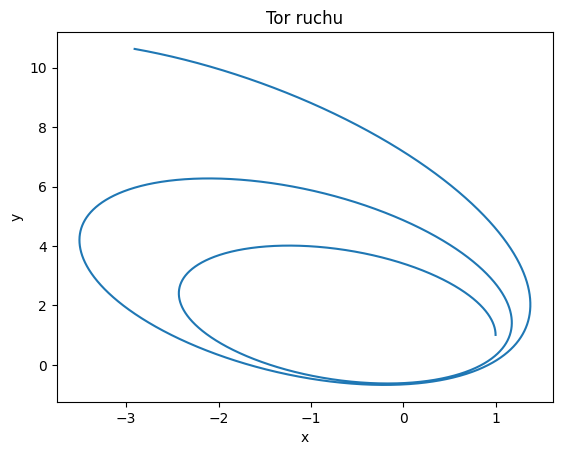
\includegraphics[scale = 0.5]{wykres1.png}
	\end{figure}

	\begin{figure}[h]
		\centering
		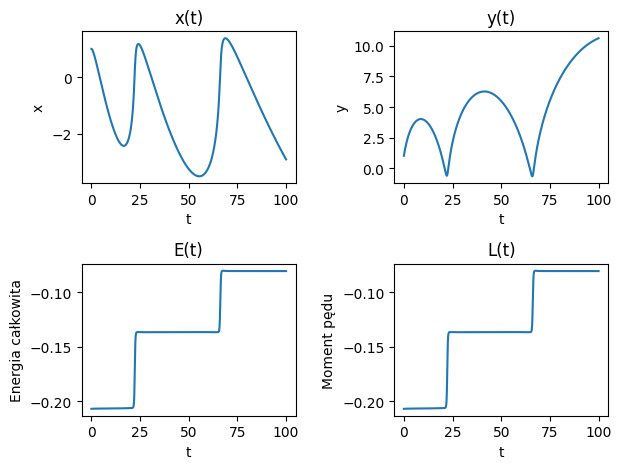
\includegraphics[scale = 0.70]{wykres2.png}
	\end{figure}


	\newpage

	\subsection*{Niejawna metoda Euler'a}

	Wzór niejawnej metody Euler'a:

	\begin{equation}
		y_{k+1} = y_k + h \cdot f(t_{k+1}, y_{k+1})
	\end{equation}

	W podanej sytuacji:

	\begin{equation}
		x_{k+1} = x_k + \Delta t \cdot f(t_{k+1}, x_{k+1})
	\end{equation}

	\begin{equation}
		x_{k+1} = x_k + \Delta t \cdot (v_{x_{k}} - \Delta t \cdot \frac{GM}{R^3} \cdot x_{k+1})
	\end{equation}

	\begin{equation}
		x_{k+1} = \frac{x_k+ \Delta t \cdot  v_{x_{k}}}{1 + (\Delta t)^2 \cdot GM \cdot R^{-3}}
	\end{equation}



	

	Analogiczne wzory zastosowano dla $y$ oraz $v_y$. Na podstawie tych czterech równań stworzono wykresy (dla $e = 0$):

	\begin{figure}[h]
		\centering
		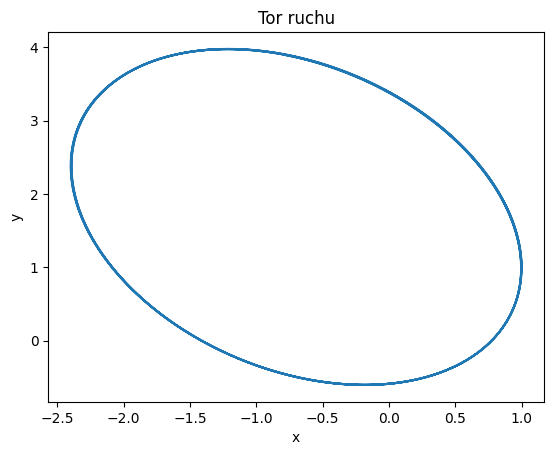
\includegraphics[scale = 0.7]{wykres3.png}
	\end{figure}

	\begin{figure}[h]
		\centering
		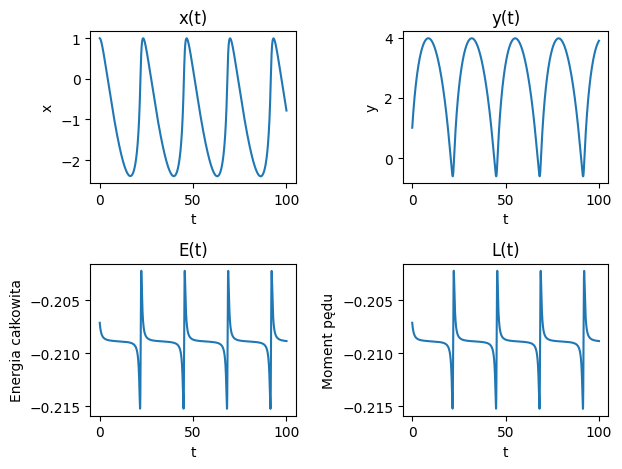
\includegraphics[scale = 0.70]{wykres4.png}
	\end{figure}

	\newpage

	\subsection*{Półjawna metoda Euler'a}

	Wzór półjawnej metody Euler'a:

	\begin{equation}
		v_{n+1} = v_n + h \cdot g(t_n, x_n)
	\end{equation}

	\begin{equation}
		x_{n+1} = x_n + h \cdot f(t_n, v_{n+1})
	\end{equation}

	W podanej sytuacji:

	\begin{equation}
		v_{x_{k+1}} = v_{x_k} - \Delta t \cdot \frac{GM}{R^3} \cdot x_k
	\end{equation}

	\begin{equation}
		x_{k+1} = x_k + \Delta t \cdot v_{x_{k+1}} 
	\end{equation}

	\newpage

	Analogiczne zależności wyprowadzono dla $y$ oraz $v_y$. Dla $e = 0$ stworzono wykresy:

	
	\begin{figure}[h]
		\centering
		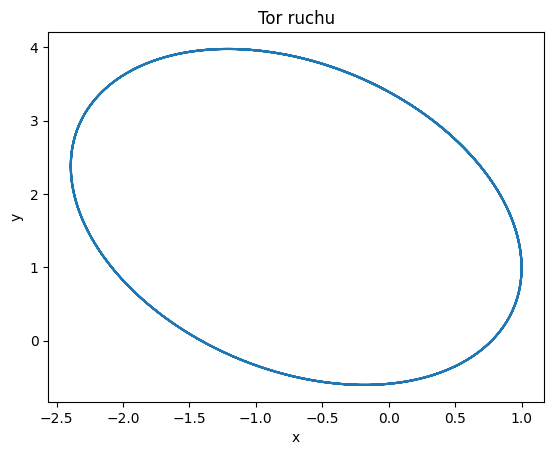
\includegraphics[scale = 0.5]{wykres5.png}
	\end{figure}

	\begin{figure}[h]
		\centering
		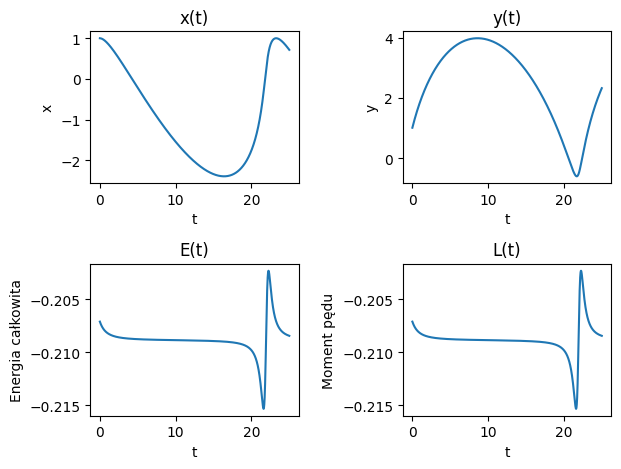
\includegraphics[scale = 0.70]{wykres6.png}
	\end{figure}

	\newpage

	\subsection*{Metoda Rungego-Kutty czwartego rzędu (RK4)}

	Wzór metody Rungego-Kutty czwartego rzędu:

	\begin{equation}
		y_{k+1} = y_k + \frac{h}{6} \cdot (k_1+2k_2+2k_3+k_4)
	\end{equation}

	\begin{equation}
		k_1 = f(t_k, y_k)
	\end{equation}

	\begin{equation}
		k_2 = f(t_k+\frac{h}{2}, y_k + \frac{hk_1}{2})
	\end{equation}

	\begin{equation}
		k_3 = f(t_k+\frac{h}{2}, y_k + \frac{hk_2}{2})
	\end{equation}

	\begin{equation}
		k_4 = f(t_k+h, y_k+hk_3)
	\end{equation}

	W podanej sytuacji:

	\begin{equation}
		x_{k+1} = x_k + \frac{\Delta t}{6} \cdot (k_1 + 2k_2+2k_3+k_4)
	\end{equation}

	\begin{equation}
		k_1 = v_k - \Delta t \cdot GM \cdot x_k \cdot R^{-3}
	\end{equation}

	\begin{equation}
		k_2 = v_k - \frac{1}{2} \Delta t \cdot GM \cdot R^{-3} \cdot \left( 3x_k + \Delta t \cdot k_1 \right)
	\end{equation}

	\begin{equation}
		k_3 = v_k - \frac{1}{2} \Delta t \cdot GM \cdot R^{-3} \cdot \left( 3x_k + \Delta t \cdot k_2 \right)
	\end{equation}

	\begin{equation}
		k_4 = v_k - \Delta t \cdot GM \cdot R^{-3} \cdot \left( 2x_k + \Delta t \cdot k_3 \right)
	\end{equation}

	\newpage

	Analogiczne zależności wyprowadzono dla $y$ oraz $v_y$. Dla $e = 0$ stworzono wykresy:

	\begin{figure}[h]
		\centering
		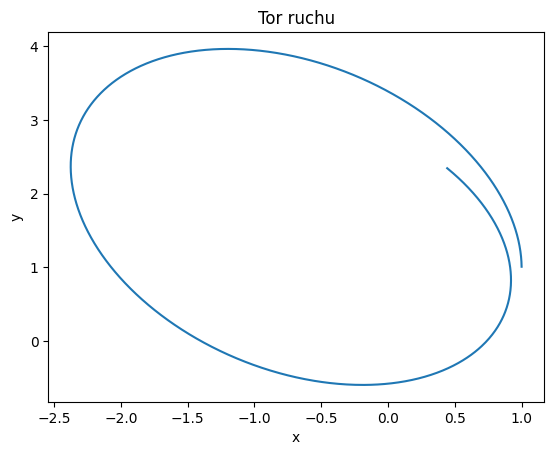
\includegraphics[scale = 0.5]{wykres7.png}
	\end{figure}

	\begin{figure}[h]
		\centering
		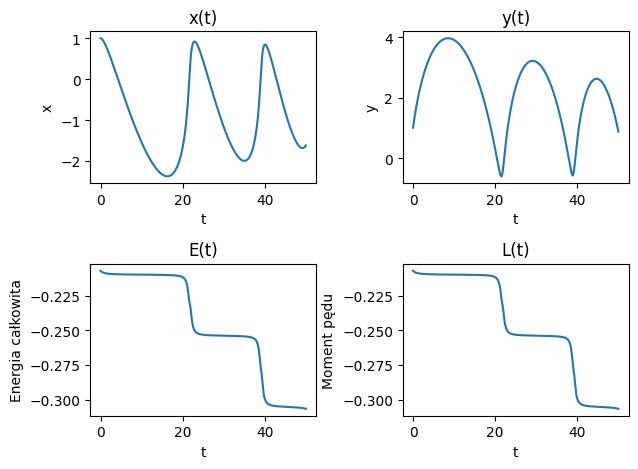
\includegraphics[scale = 0.70]{wykres8.png}
	\end{figure}




	

	
	
	
\end{document}